\subsection{Algorithm}

The algorithm is based on two main groups. A list of \textit{basic functions} and a list of \textit{binary operators} to combine them. They are shown in table \ref{tab:BasicGroups}.
\begin{table}[h!]
	\centering
	\begin{tabular}{c|ccccccccc}
		\textbf{Basic functions} & \( 1 \) & \( \exp(x) \) & \( \sin(x) \) & \( x^2 \) & \( \tan(x) \) & \( \log(x) \) & \( |x| \) & \( a \) & \( x \) \\
		\hline
		\textbf{Basic operators} & \(a+b \) & \(a-b \) & \(a \cdot b \) & $\frac{a}{b}$ & \( a^b \) & & & &
	\end{tabular}
	\caption{Basic functions and binary operators}
	\label{tab:BasicGroups}
\end{table}\\The idea is to choose basic functions and combine them with some operators. Since this could lead to infinite possibilities it was necessary to do some design choices.\\
\\
\textbf{Representation}\\
The functions are represented as \textit{Computational Graphs}. \Fig~\ref{fig:ComputationalGraph} gives an example of such a representation. It refers to the function \(f(x) = \sin(x) \cdot e^x - x\) of \Fig~\ref{fig:GeneralIdea}.
\begin{figure}[h!]
	\centering
	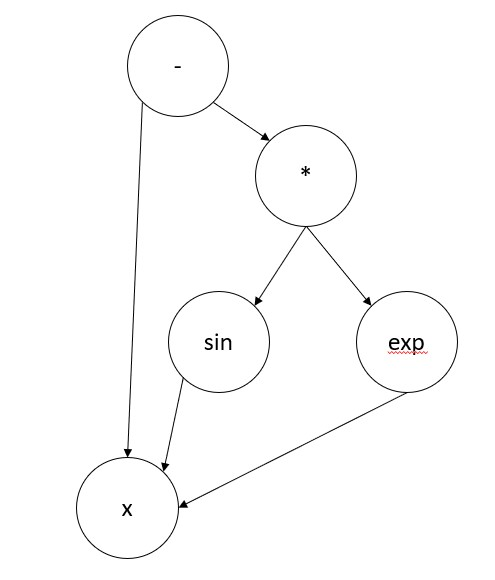
\includegraphics[width=0.25\linewidth]{./ImageFiles/Data Generation/ComputationalGraph}
	\caption{Computational graph example}
	\label{fig:ComputationalGraph}
\end{figure}\\
\textbf{Simplifications}\\
The first simplification is referred to the maximum number of children at each node, which is two. The result is a binary graph.\\
The second simplification is the graph depth. This limits the possible number of functions that can be generated. It is kept less or equal to three. The depth is directly proportional to the function's complexity. Here are some examples for different complexity levels.\\
\begin{table}[h!]
\centering
\begin{tabular}{c|c|c}
	\textbf{Complexity level 1} & \textbf{Complexity level 2} & \textbf{Complexity level 3}\\
	\hline
	$f(x) = \sin(x) + x$ & $f(x) = \tan(\sin(x) + x)$ & $f(x) = \tan(\sin(x)+x) x^2$\\
	$f(x) = \log(\sin(x))$ & $f(x) = \log(\sin(x) x^2)$ & $f(x) = \frac{\log(\sin(x))}{x}$\\
	$f(x) = \frac{e^x}{x^2}$ & $f(x) = |\frac{e^x}{\sin(x)}|$ & $f(x) = |\frac{e^x}{x} - \frac{a}{x}|$
		\end{tabular}
		\caption{Complexity Levels}
		\label{tab:Complexity Levels}
\end{table}\\
\textbf{Generation}\\
The generation is made with different levels of complexity to guarantee a fair distribution in the dataset. More precisely, 10\% is depth 1, 30\% depth 2 and 60\% depth 3. The precentage is proportional to the number of possible resulting functions.\\
Two datasets are generated, a reduced one with 2000 samples to do preliminary training and a larger one with 50000 samples.\\
\\
\textbf{Adjustments}\\
Some further adjustments were made to the algorithm in order to get better datasets. The first problem was the huge presence of constant functions, e.g. a function like $f(x) = \sin(x) - \sin(x)$ is just a konstant. These simple solutions were filtered out to reduce the redundancy of our dataset.\\
An different problem was given by equivalent representations, e.g. $f(x) = x + x$ and $f(x) = 2x$. They are the same functions with different representation. This could lead to confusion in the model. We were not able to deleted all these combinations but we strongly mitigated them.